\section{Grid}\label{sec:grid}

We will estimate values of $J_D$ at nodes with uniform spacing, $\delta$ in both $x$ and $y$ directions.  Though the choice of uniform spacing is not mandatory for this approach, it simplifies matters while sacrificing little generality.  Our problem may be said to contain $N_n$ nodes forming $N_e$ $\delta\times \delta$ square elements when the array of nodes contains $N_x$ $x$-values and $N_y$ $y$-values, and
\begin{align}
N_n &= N_x N_y\\
N_e &= (N_x -1)(N_y -1).
\end{align}
Nodes may be indexed either sequentially (using index $n$) from left-to-right and then bottom-to-top, or by $x$- and $y$-indices (using indices $i$ and $j$).  The equivalent indices may be found
\begin{align}
n &= jN_x + i\\
j &= \mathrm{floor}(n/N_x)\\
i &= n - jN_x
\end{align}
when $n \in [0, N_n-1]$, $i \in [0, N_x-1]$, and $j \in [0, N_y-1]$.  

This indexing scheme is depicted in Figure \ref{fig:indexing} with six columns and five rows of nodes.
\begin{figure}
\begin{center}
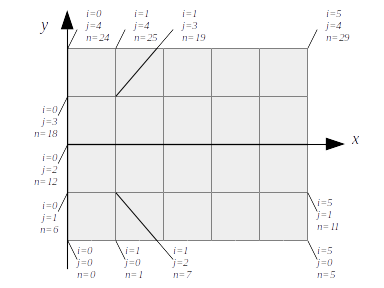
\includegraphics{indexing}
\caption{An example demonstrating the indexing schemes for nodes.}\label{fig:indexing}
\end{center}
\end{figure}

We will take $\X$ to be a vector of all node values for $J_D$, which can be indexed either in sequential order, $X_n$, or by $x$- and $y$-indices, $X_{i,j}$.  Elements are numbered to match the index of the node in the bottom-left corner, so that $X_n$ is the bottom-left value of element $(n)$.  However, it is important to note that the top- and right-most elements cannot be evaluated since they will be missing nodes.

Once we have applied some interpolation scheme for approximating values of $J_D$, the integral of Equation \ref{eqn:ek} will be expressible as a vector dot product,
\begin{align}
\int_0^R J_D(r, d, \theta)\d r = \Lam(R, d, \theta) \cdot \X \label{eqn:lambda}
\end{align}
Though we have not yet established a means for calculating $\Lam$, when our choices for all $\X$ are optimal,
\begin{align}
0 &= \frac{\partial E^2}{\partial X_n} \nonumber\\
& = \sum_k 2 e_k\frac{\partial e_k}{X_n} \nonumber\\
&= \sum_k \left(-I_k + \pi D_w \int_0^R J_D(r, d_k, \theta_k) \mathrm{d}r \right)\int_0^R \frac{\partial J_D(r, d_k, \theta_k)}{\partial X_n} \d r\nonumber\\
&= -\sum_k I_k \Lam_k + \pi D_w \left[\sum_k \Lam_k \Lam_k\right] \cdot \X \label{eqn:lsqr}
\end{align}

This represents a matrix inversion problem for the calculation of the node values, $\X$.  All that remains is to develop a means of calculating the interpolation vectors, $\Lam_k$ = $\Lam(R,d_k,\theta_k)$, for a wire of radius, $R$, center of rotation, $d_k$, and angle, $\theta_k$.  In this way, there is a separate $\Lam$ vector for each raw measurement, $k$.

\subsection{Interpolation}\label{sec:interpolate}

Each element is a finite domain in $x,y$ space over which we may estimate the continuous function, $J_D$, at a point, $\p = [x,y]^T$, by linear interpolation of the node values.  
\begin{align}
J_D(\p) &= \nonumber\\
 &X_{i,j}\,\phi_{00} (\p) + X_{i+1,j}\,\phi_{10} (\p) + \dots\nonumber\\
 &X_{i,j+1}\,\phi_{01} (\p) + X_{i+1,j+1}\,\phi_{11} (\p)
\end{align}
when the $\phi$ functions are interpolation functions which we must define.  Note that this is only valid when $\p$ lies within the element, so $x_i \le x \le x_{i+1}$ and $y_j \le y \le y_{j+1}$.

A formulation of the interpolation functions is facilitated by using a scaled coordinate system, $\hat{x} = (x-x_i)/(x_{i+1} - x_i)$, $\hat{y} = (y-y_j)/(y_{j+1} - y_j)$, or
\begin{align}
[\hat{x}, \hat{y}]^T = \hat{\p} = \frac{\p - \p_{i,j}}{\delta},
\end{align}
This constitutes a coordinate system with its origin at the bottom-left most node in the element (node $n$ or equivalently node $i,j$) extending to $\hat{x}=1$ at its right-most, and $\hat{y} = 1$ at its top most extent.  These interpolation functions are \emph{only} valid in that range.

For the interpolated values for $J_D$ to agree with the node values at the verticies, each interpolation function must be one at its own node and zero at the other three.  This implies four constraints on each interpolation function, permitting a four-term $x,y$ polynomial.  Using the element-scaled coordinate system, the resulting interpolation functions are
\begin{subequations}
\begin{align}
\phi_{00} &= (1-\hat{x})(1-\hat{y})\\
\phi_{10} &= \hat{x}(1-\hat{y})\\
\phi_{01} &= (1-\hat{x})\hat{y}\\
\phi_{11} &= \hat{x}\hat{y}
\end{align}
\end{subequations}
and may be more compactly written $\phi(\hat{\p})$.  Note that each $\phi$ is unity when $\hat{\p}$ is at its respective node, but declines to zero at all other nodes.

\subsection{Line Segments}\label{sec:segments}

Constructing the wire's path in space and the bounds on an element's regime in space is accomplished by defining line segments.  In the case of elements, the four segments defining their boundary are simply defined by the segments connecting the nodes.  In the case of the wire, the wire may be imagined to extend a radius, $R$, from the center of rotation at some angle relative to the $x$-axis.

It is convenient to define a line segment by a starting point, $\p_0$, and a direction, $\Delta \p$.  Therefore, the line segment is defined as
\begin{align}
\p(s) = \p_0 + s \Delta \p \hspace{2em} \forall \ s\in[0,1].
\end{align}
Negative values of $s$ and values greater than 1 represented points projected beyond the bounds of the line segment.  The value of $s$ is related to the distance along the segment, $r$, by
\begin{align}
r = s \| \Delta \p \|.
\end{align}

To calculate the location of an intersection between two line segments, $a$ and $b$,
\begin{align}
\p_a(s_a) &= \p_{0,a} + s_a \Delta \p_a\nonumber\\
\p_b(s_b) &= \p_{0,b} + s_b \Delta \p_b\nonumber,
\end{align}
we need only set the points $\p_a$ and $\p_b$ equal and solve for $s_a$ and $s_b$.  The problem is equivalent to
\begin{align}
\p_{0,b} - \p_{0,a} &= \left[\Delta \p_a,\ -\Delta \p_b\right] \cdot \left[s_a,\ s_b\right]^T
\end{align}
or, in terms of the individual $x$ and $y$ components,
\begin{align}
\left[\begin{array}{c}
x_{0,b} - x_{0,a}\\
y_{0,b} - y_{0,b}
\end{array}\right] &= 
\left[\begin{array}{cc}
\Delta x_a & -\Delta x_b\\
\Delta y_a & -\Delta y_b
\end{array}\right]\left[\begin{array}{c}
s_a \\
s_b
\end{array}\right]
\end{align}

There are five cases that can occur when searching for segment intersections:
\begin{enumerate}
\item If the determinant of the matrix, $\Delta x_b \Delta y_a - \Delta x_a \Delta y_b$ is zero, then the segments are parallel, and there is no solution,
\item If $0 \le s_a \le 1$ and $0 \le s_b \le 1$ then the segments intersect,
\item If $0 \le s_a \le 1$ but not $s_b$, then a projection of segment $b$ intersects segment $a$,
\item If $0 \le s_b \le 1$ but not $s_a$, then a projection of segment $a$ intersects segment $b$,
\item If neither $s_a$ nor $s_b$ is between 0 and 1, then only the projections of the segments intersect.
\end{enumerate}

For line segments expressed within an element's dimensionless coordinate system,
\begin{align}
\hat{\p}(s) &= \frac{\p(s) - \p_n}{\delta} = \hat{\p}_0 + s\Delta \hat{\p}\\
\hat{\p}_0 &= \frac{\p_0 - \p_n}{\delta}\nonumber\\
\Delta \hat{\p} &= \frac{\Delta \p}{\delta}\nonumber.
\end{align}
This alternate formulation for a line segment is simply re-scaled by the elements size and offset by its bottom-left element's coordinates.

\subsection{Calculating $\Lam$}\label{sec:lambda}

Equation \ref{eqn:lsqr} reduces the deconvolution problem to a matrix inversion in terms of sums of $\Lam_k = \Lam(R,d_k,\theta_k)$ defined in Equation \ref{eqn:lambda}.  Here, we use the interpolation functions to calculate $\Lam$ for the $k$ data point with the disc center of rotation at $x=-d_k$, and the wire at an angle, $\theta_k$.  For each such wire location, elements may fall into three categories:
\begin{enumerate}
\item Elements through which the wire does not pass,
\item Elements with the wire passing through two faces,
\item An element with the wire passing through only one face.
\end{enumerate}
The first will constitute the vast majority of elements for any given wire location and do not contribute to the integral.  In this approach, we will consider each element that contains a segment of the wire, and we will accumulate their contributions to $\Lam$.

The integration of $J_D$ over only the $n$ element will contain contributions from the four nodes that form its limits,
\begin{align}
\int_{(n)} J_D \mathrm{d} r &= X_{i,j} \int_{(n)} \phi_{00} \mathrm{d} r + X_{i+1,j} \int_{(n)} \phi_{10} \mathrm{d} r + \ldots \nonumber\\
&\ X_{i,j+1} \int_{(n)} \phi_{01} \mathrm{d} r + X_{i+1,j+1} \int_{(n)} \phi_{11} \mathrm{d} r \label{eqn:intJD:element}
\end{align}

Note that we have been quite deliberately vague with regard to the bounds on the integrals over $r$.  Once we have isolated a line segment, $\p(s)$, within element $n$, each integral may be rescaled to be in terms of $s$,
\begin{align}
\int_{(n)} \phi \mathrm{d}r = \|\Delta\p\| \int_0^1 \phi(\hat{p}(s)) \mathrm{d} s.
\end{align}
since $\d r = \|\Delta \p\| \d s$.

So, the four interpolation function integrals are
\begin{subequations}
\begin{align}
\Phi_{00} &= \int_0^1 \phi_{00}(s) \mathrm{d}s = \int_0^1 (1-\hat{x}_0 - s\Delta\hat{x})(1-\hat{y}_0-s\Delta\hat{y})\mathrm{d}s\nonumber\\
 &= \frac{\Delta \hat{x} \Delta \hat{y}}{3} - \frac{\Delta \hat{x} (1-\hat{y}_0)}{2} - \frac{\Delta \hat{y} (1-\hat{x}_0)}{2} + (1-\hat{x}_0)(1-\hat{y}_0)\\
\Phi_{10} &= \int_0^1 \phi_{10}(s) \mathrm{d}s = \int_0^1 (\hat{x}_0 + s\Delta\hat{x})(1-\hat{y}_0-s\Delta\hat{y})\mathrm{d}s\nonumber\\
 &= -\frac{\Delta \hat{x} \Delta \hat{y}}{3} + \frac{\Delta \hat{x} (1-\hat{y}_0)}{2} - \frac{\Delta \hat{y} \hat{x}_0}{2} + \hat{x}_0(1-\hat{y}_0)\\
\Phi_{01} &= \int_0^1 \phi_{01}(s) \mathrm{d}s = \int_0^1 (1 - \hat{x}_0 - s\Delta\hat{x})(\hat{y}_0+s\Delta\hat{y})\mathrm{d}s\nonumber\\
 &= -\frac{\Delta \hat{x} \Delta \hat{y}}{3} - \frac{\Delta \hat{x} \hat{y}_0}{2} + \frac{\Delta \hat{y} (1-\hat{x}_0)}{2} + (1-\hat{x}_0)\hat{y}_0\\
\Phi_{11} &= \int_0^1 \phi_{11}(s) \mathrm{d}s = \int_0^1 (\hat{x}_0 + s\Delta\hat{x})(\hat{y}_0+s\Delta\hat{y})\mathrm{d}s\nonumber\\
 &= \frac{\Delta \hat{x} \Delta \hat{y}}{3} + \frac{\Delta \hat{x} \hat{y}_0}{2} + \frac{\Delta \hat{y} x_0}{2} + \hat{x}_0 \hat{y}_0
\end{align}
\end{subequations}

Finally, we may construct $\Lam$ in terms of these $\Phi$ formulae.  Here, the contribution to each $\Lam$ element from only element $n$ is
\begin{subequations}\label{eqn:lambda:n}
\begin{align}
\Lambda_{i,j}^{(n)} &= \|\Delta \p\| \Phi_{00}\\
\Lambda_{i+1,j}^{(n)} &= \|\Delta \p\| \Phi_{10}\\
\Lambda_{i,j+1}^{(n)} &= \|\Delta \p\| \Phi_{01}\\
\Lambda_{i+1,j+1}^{(n)} &= \|\Delta \p\| \Phi_{11}
\end{align}
\end{subequations}
and zero otherwise.  The total $\Lam$ vector is constructed by summing these values contributed from all the elements.
\begin{align}
\Lambda_{i,j} = \sum_n \Lambda_{i,j}^{(n)}
\end{align}
